\documentclass[10pt,a5paper,twoside]{book}
\usepackage{geometry}
\usepackage[T1]{fontenc}
\usepackage[english]{babel}
\usepackage{libertine}
\usepackage[scaled=0.95]{inconsolata}
\usepackage{microtype}
\SetTracking
  [ spacing = {25*,166, } ]
  { encoding = *,
    shape = sc }
  { 50 }
\usepackage{xstring}
\usepackage{graphicx}
\usepackage{wallpaper}
\usepackage{chngcntr}
\usepackage{listings}
\lstset{
  basicstyle=\normalsize\ttfamily\lst@ifdisplaystyle\footnotesize\fi,
  backgroundcolor=\color{black!6},
  rulecolor=\color{black!25},
  frame=single,
  breaklines=true,
  breakatwhitespace=true,
  keepspaces=true,
  columns=fixed,
  showspaces=false,
  showstringspaces=false,
  xleftmargin=3.4pt,
  xrightmargin=3.4pt,
  framerule=0.4pt,
  belowskip=\smallskipamount,
  language=Perl
}

% Environment to show command-line
\lstnewenvironment{shell}
  {\lstset{morecomment=[l]{cpan>},
           morecomment=[l]{$},
           commentstyle=\bfseries,
           breaklines=true,
           breakatwhitespace=false,
           breakindent=0pt}}
  {}

\usepackage{titlesec}
\usepackage{titletoc}

% Headers and footers
\usepackage{fancyhdr}
\renewcommand{\headrulewidth}{0pt}
\fancypagestyle{main}{%
  \fancyhf{}
  \fancyhead[CO,CE]{\small\nouppercase{\leftmark}}
  \fancyhead[LE,RO]{\sffamily\bfseries\thepage}}
\fancypagestyle{plain}{%
  \fancyhead{}
  \fancyfoot[LE,RO]{\sffamily\bfseries\thepage}}
\pagestyle{main}
\renewcommand{\chaptermark}[1]{%
  \markboth{\sffamily\textsc{\lsstyle\chaptername} \thechapter\ \// #1}{}}
% To have a blank page completely blank before a chapter page
\makeatletter
\def\cleardoublepage{\clearpage\if@twoside \ifodd\c@page\else
  \hbox{}
  \thispagestyle{empty}
  \newpage
  \if@twocolumn\hbox{}\newpage\fi\fi\fi}
\makeatother

\usepackage{hyperref}
\let\urlfromhyperref\url
\addto\extrasenglish{%
  \renewcommand{\chaptername}{Day}%
  \renewcommand{\chapterautorefname}{Day}%
}
\PassOptionsToPackage{hyphens}{url}

\titleformat{\chapter}[display]
    {\normalfont\rmfamily\filcenter}
    {\Large\scshape\lsstyle \chaptername{} \thechapter}
    {0.5pc}
    {\LARGE\itshape}
\titlespacing*{\chapter}
  {0pt}{*-3}{*10}

\titleformat{\section}
  {\normalfont\bfseries}
  {\llap{\thesection\hspace{1.5ex}}}
  {0pt}
  {}
\titlespacing*{\section}
  {0pt}{*2}{*1}

% Table of content
\titlecontents{chapter}
  [0pt] % left
  {\addvspace{3.6pt}} % above
  {\bfseries{\scshape\lsstyle\chaptername\ \thecontentslabel\ /\ }} % before with label
  {\bfseries \thecontentslabel} % before without label
  {\titlerule*[0.5pc]{.}\contentspage} % filler and page
  [] % after
\titlecontents*{section}
  [0pt]
  {\small\itshape}
  {}
  {}
  {\hspace{0.5em}\thecontentspage}
  [~\textbullet\ ]

% Remove the numbers from section headings
\setcounter{secnumdepth}{0}

% Continuous figure numbering
\counterwithout{figure}{chapter}

\graphicspath{{images/}}

% Create a footnote for each href link
\let\oldhref\href
\renewcommand{\href}[2]{%
  % Every Perl developper knows where to find documentation for Perl modules
  % so there is no need to waste space in the footnote
  \IfSubStr{#1}{cpan.org}{#2}{#2\footnote{\urlfromhyperref{#1}}}%
}

\usepackage[strict]{changepage}
\newenvironment{note}
  {\medskip\begin{adjustwidth}{\parindent}{\parindent}%
    % Why -2pt is needed ?
    \makebox[-2pt][r]{\scshape\lsstyle Note\space}\small}%
  {\end{adjustwidth}\medskip}

%
% Typographical conventions
%
\newcommand*{\sourceFont}{\ttfamily\footnotesize}
\newcommand*{\inlineSourceFont}{\normalsize\ttfamily}
\newcommand*{\urlFont}{\itshape}
\renewcommand*{\UrlFont}{\itshape}
\newcommand*{\fileFont}{\itshape}
\newcommand*{\moduleFont}{\ttfamily}
\newcommand*{\programFont}{\itshape}
% url
\DeclareUrlCommand\url{\def\UrlFont{\urlFont}}
% filename
\DeclareUrlCommand\file{\def\UrlFont{\fileFont}}
% Module or distribution name
% Hyphenation can occur after :: or at |
% Usage: \module{Plack::Mid|dle|wa|re::Ses|sion}
\makeatletter
\DeclareUrlCommand\module{%
  \def\UrlFont{\moduleFont}%
  \def\UrlBigBreaks{\do\:}%
  \g@addto@macro\UrlSpecials{\do\|{\allowbreak}}%
}
\makeatother
% Program name
\newcommand*{\program}[1]{{\programFont#1}}

% Command-line switch
\newcommand*{\switch}[1]{\textit{#1}}

% How to include an SVG image in LaTeX, Johan B. C. Engelen
% http://mirrors.ircam.fr/pub/CTAN/info/svg-inkscape/InkscapePDFLaTeX.pdf
\newcommand{\executeiffilenewer}[3]{%
  \ifnum\pdfstrcmp{\pdffilemoddate{#1}}%
  {\pdffilemoddate{#2}}>0%
  \immediate\write18{#3}\fi%
}
\newcommand{\includesvg}[2][]{%
  \executeiffilenewer{#2.svg}{#2.pdf}%
  {inkscape -z -D --file=#2.svg --export-pdf=#2.pdf --export-pdf}%
  \includegraphics[#1]{#2.pdf}%
}

\newcommand{\downloadcoverphoto}[2]{%
  \IfFileExists{images/#1}{}{\immediate\write18{wget -O images/#1 "#2"}}%
}

\newcommand{\inputperl}[1]{%
  \executeiffilenewer{codes/#1}{build/#1}%
  {perltidy codes/#1 -pro=.perltidyrc -l=63 > build/#1}%
  \executeiffilenewer{.perltidyrc}{build/#1}%
  {perltidy codes/#1 -pro=.perltidyrc -l=63 > build/#1}%
  \lstinputlisting{build/#1}
}

\frenchspacing

\begin{document}

\title{Plack Handbook}
\author{Tatsuhiko Miyagawa}
\date{}

\frontmatter

\begin{titlepage}
  \newgeometry{margin=2cm}
  \setlength{\wpXoffset}{0cm}
  \setlength{\wpYoffset}{-2cm}
  \downloadcoverphoto{cover-a5.jpg}{https://lut.im/JDt1SkPJ/Ug7omIxq?dl}
  \ThisCenterWallPaper{1}{cover-a5.jpg}  
  \null
  {\fontsize{60}{72}\selectfont\bfseries\color{black}\hfill Plackup}\\[1.2\baselineskip]
  {\fontsize{60}{72}\selectfont\bfseries\color{lightgray}\hfill Handbook}
  \vfill
  {\LARGE\color{black}\hfill\itshape Tatsuhiko Miyagawa}
\end{titlepage}




\thispagestyle{empty}
\null
\vfill
\begin{center}
  \small
  \textbf{Plackup Handbook}

  \bigskip
  
  Copyright \copyright{} 2009--2012 by Tatsuhiko Miyagawa

  \bigskip

  The content of this book is licensed under a Creative Commons Attribution-NonCommercial 3.0 Unported 
  \url{http://creativecommons.org/licenses/by-nc/3.0/}

  \medskip

  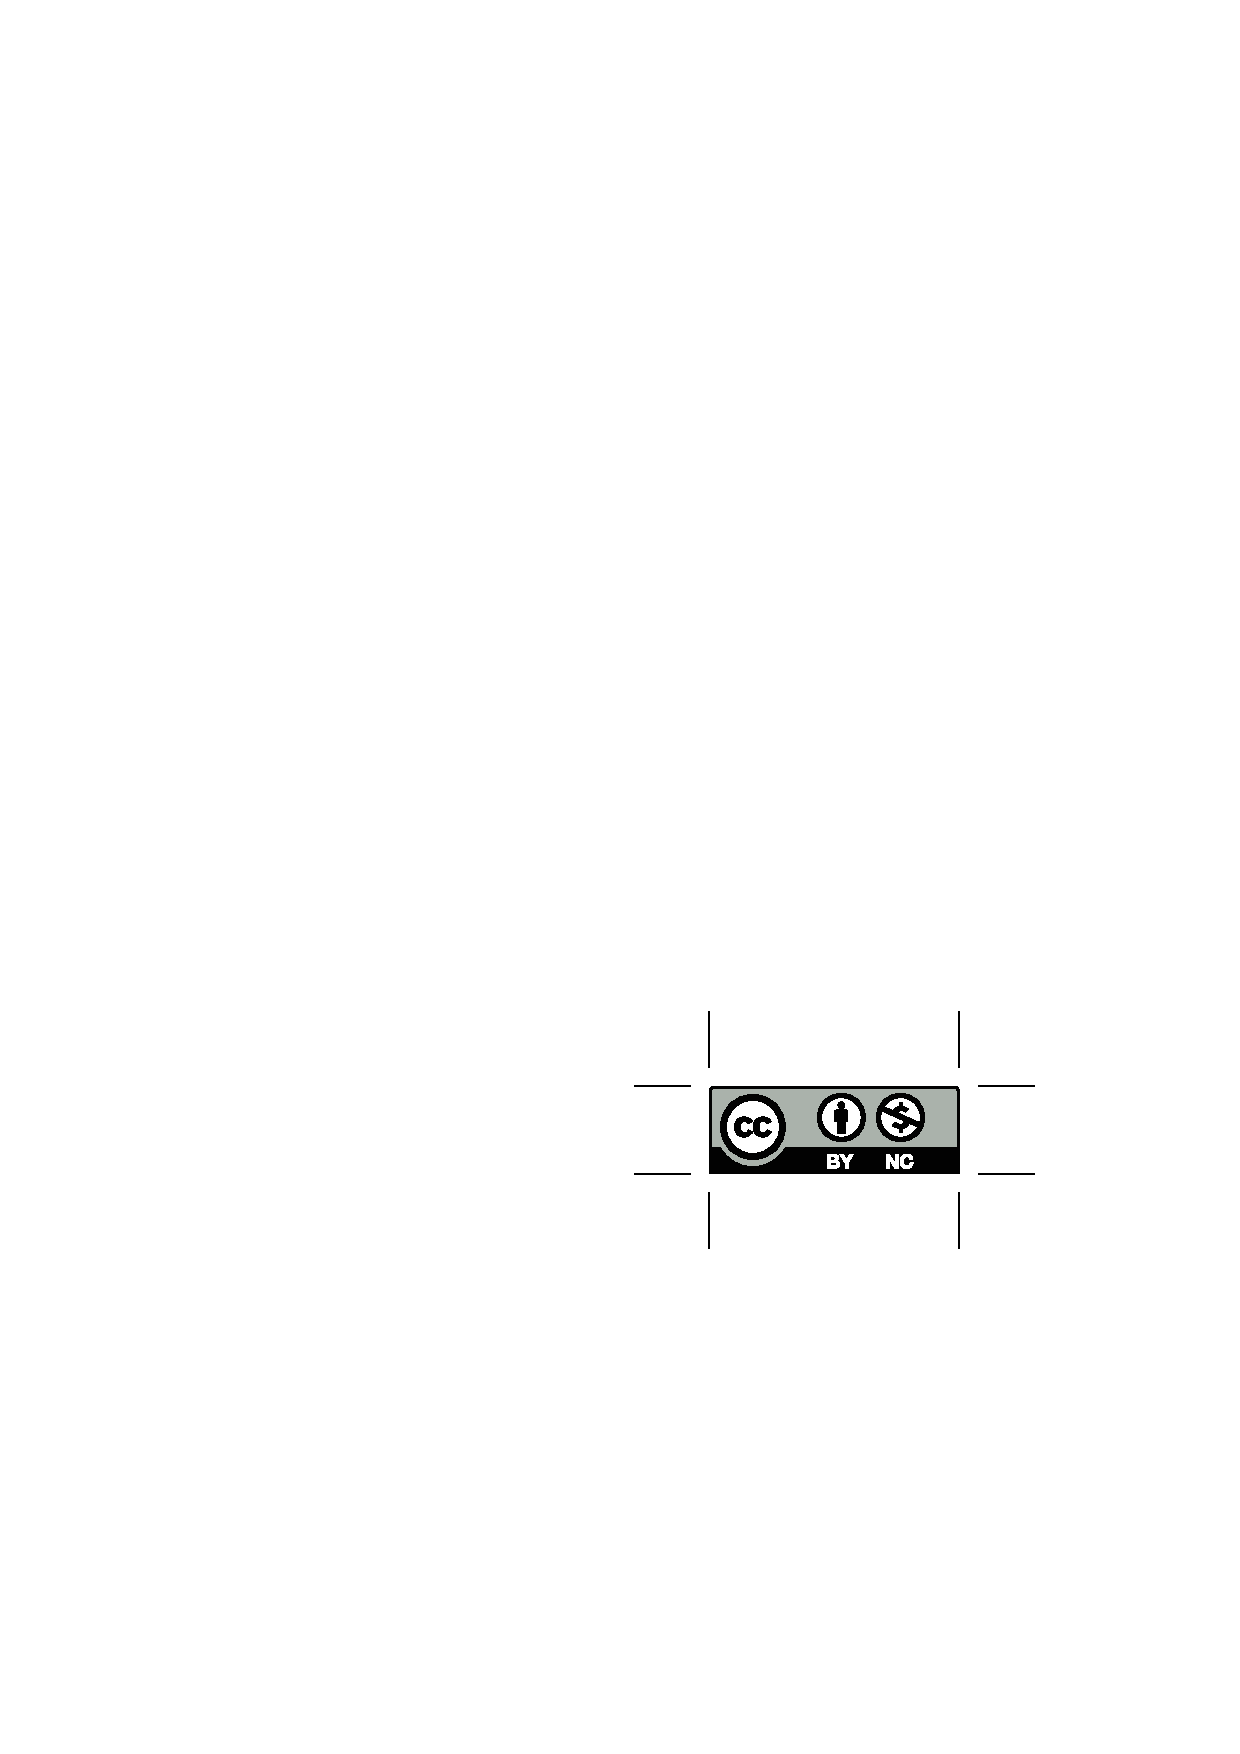
\includegraphics[width=2cm]{images/cc-by-nc}

  \bigskip

  Cover photography:
  
  \textit{Long Exposure in Yurikamome (Daiba, Tokyo, Japan)} by t-mizo
  \url{https://www.flickr.com/photos/tmizo/8330024896/}
 
  Licensed under a Creative Commons Attribution 2.0
  \url{http://creativecommons.org/licenses/by/2.0/}

 
\end{center}





\tableofcontents

\chapter{Introduction}\label{introduction}

This little handbook is based on the content of the
\href{http://advent.plackperl.org/}{Plack Advent Calendar} website. The
calendar had 24 useful short posts explaining the concept of PSGI and
how to adapt existing web applications to Plack.

The calendar was so successful it's been considered a canonical
reference for many beginners trying to learn Plack and for web framework
authors trying to adapt their code to work with PSGI.

But the content was written 3 years ago and some of it is a little
dated. In this book I tried to get it correct and up-to-date, and it
will continue to be updated as we find errata and get feedback from the
reader community.

Raw source code of the book, in Markdown format, is available on
\href{https://github.com/miyagawa/plack-handbook}{GitHub repository}
under the Creative Commons license. See the \file{LICENSE} file for details.

\begin{flushright}
  Tatsuhiko \textsc{\lsstyle Miyagawa} \\
  \textit{September 2012}
\end{flushright}



\mainmatter

\chapter{Getting Plack}\label{day-1-getting-plack}

The most important step to get started is to install
\href{http://search.cpan.org/dist/Plack}{Plack} and other utilities.
Because PSGI and Plack are just normal Perl module distributions the
installation is easy: just launch your CPAN shell and type:

\begin{shell}
cpan> install PSGI Plack
\end{shell}

\href{http://search.cpan.org/dist/PSGI}{PSGI} is a specification
document for the PSGI interface. By installing the distribution you can
read the documents in your shell with the \lstinline!perldoc PSGI! or
\lstinline!perldoc PSGI::FAQ! commands. Plack gives you the standard
server implementations, core middleware components, and utilities like
\program{plackup} and \module{Plack::Test}.

Plack doesn't depend on any non-core XS modules so with any Perl
distribution later than 5.8.1 (which was released more than 6 years
ago!) it can be installed very easily, even on platforms like Win32 or
Mac OS X without developer tools (i.e.~C compilers).

If you're a developer of web applications or frameworks (I suppose you
are!), it's highly recommended you install the optional module bundle
\href{http://search.cpan.org/dist/Task-Plack}{\module{Task::Plack}} as well. The
installation is as easy as typing:

\begin{shell}
cpan> install Task::Plack
\end{shell}

You will be prompted with a couple of questions depending on your
environment. If you're unsure whether you should or should not install,
just type return to select the default. You'll get optional XS speedups
by default, while other options like non-blocking environments are
disabled by default.

Start reading the documentation with \lstinline!perldoc Plack! to get
prepared.



\chapter{Hello World}\label{day-2-hello-world}

The first program you write in any programming language is the one that
prints ``Hello World''. Let's follow that tradition for PSGI as well.

\begin{note}
  Today's code is written to a raw PSGI interface to help
you understand what's going on. In reality you should never have to do
this unless you're a web application framework developer. Instead you
should use one of the \href{http://plackperl.org/\#frameworks}{existing
frameworks that supports PSGI}.
\end{note}

\section{Hello, World}\label{hello-world}

Here's the minimal code that prints ``Hello World'' to the client:

\inputperl{day2-1.pl}

A PSGI application is a Perl subroutine reference (a coderef) and is
usually referenced as \lstinline!$app! (it could be named anything
obviously). It takes exactly one argument \lstinline!$env! (which is not
used in this code) and returns an array ref containing status, headers,
and body. That's it.

Save this code in a file named \file{hello.psgi} and then use the
\program{plackup} command to run it:

\begin{shell}
$ plackup hello.psgi
HTTP::Server::PSGI: Accepting connections at http://0:5000/
\end{shell}

The \program{plackup} command runs your application with the default HTTP server
\module{HTTP::Ser|ver::PSGI} on localhost port 5000. Open the URL
\url{http://127.0.0.1:5000/} and you should see the ``Hello World'' page.

\section{Give me something
different}\label{give-me-something-different}

The ``Hello World'' program is the simplest code imaginable. We can do more here. Let's
read and display the client information using the PSGI environment hash:

\inputperl{day2-2.pl}

This code will display the remote address using the PSGI environment
hash. It will normally be 127.0.0.1 if you're running the server on your
localhost. The PSGI environment hash contains lots of information about
an HTTP connection like incoming HTTP headers and request paths, much
like the CGI environment variables.

Want to display something that isn't just text? We can do this by
reading a file:

\inputperl{day2-3.pl}

This app would serve \file{favicon.ico} if the request path looks like
\url{/favicon.ico}, the ``Hello World'' page for requests to the root (\url{/}) and
otherwise a~404. You can see that a Perl filehandle (\lstinline!$fh!) is
a valid PSGI response, and you can use any valid HTTP status code for a
response.



\chapter{Using plackup}\label{day-3-using-plackup}

In the
\href{http://advent.plackperl.org/2009/12/day-2-hello-world.html}{Day 2}
article I used the \program{plackup} command to run the Hello World PSGI
application.

The script \program{plackup} is a command line launcher of PSGI applications inspired by
Rack's rackup command. It can be used to run any PSGI application saved
in a \file{.psgi} file with one of the PSGI web server backends using Plack
handlers. The usage is simple: just pass a \file{.psgi} file path to the
command:

\begin{shell}
$ plackup hello.psgi
HTTP::Server::PSGI: Accepting connections at http://0:5000/
\end{shell}

You can actually omit the filename if you're trying to run the file
named \file{app.psgi} in the current directory.

The default backend is chosen using one of the following methods:

\begin{itemize}
\itemsep1pt\parskip0pt\parsep0pt
\item
  If the environment variable \lstinline!PLACK_SERVER! is set it is
  used.
\item
  If some environment specific variable like
  \lstinline!GATEWAY_INTERFACE! or \lstinline!FCGI_ROLE! is set the
  backend for CGI or FCGI is used accordingly.
\item
  If the loaded \lstinline!.psgi! file uses a specific event module like
  \module{Any|Event}, \module{Co|ro} or \module{POE} the equivalent and most appropriate backend is
  chosen automatically.
\item
  Otherwise, fallback to the default ``Standalone'' backend implemented
  in the \module{HTTP::Ser|ver::PSGI} module.
\end{itemize}

You can also specify the backend yourself from the command line using
the \switch{-s} or \switch{{-}{-}server} switch:

\begin{shell}
$ plackup -s Starman hello.psgi
\end{shell}

By default the \program{plackup} command enables three middleware components to
aid development: \module{Lint}, \module{AccessLog}, and \module{StackTrace}. You can disable them
with the \switch{-E} (or \switch{{-}{-}environment}) switch:

\begin{shell}
$ plackup -E production -s Starman hello.psgi
\end{shell}

In the case that you really want to use the \lstinline!development!
Plack environment but want to disable the default middleware there is
the \switch{{-}{-}no-default-middleware} option.

Other command line switches can be passed to the server. You can specify
the server listen port with:

\begin{shell}
$ plackup -s Starlet --host 127.0.0.1 --port 8080 hello.psgi
Plack::Handler::Starlet: Accepting connections at http://127.0.0.1:8080/
\end{shell}
%
or specify the unix domain socket the FCGI backend should listen on
with:

\begin{shell}
$ plackup -s FCGI --listen /tmp/fcgi.sock app.psgi
\end{shell}

For more options for \program{plackup}, run \lstinline!perldoc plackup! from the
command line. You'll see more \program{plackup} options and hacks tomorrow as
well.



\chapter{Reloading applications}\label{day-4-reloading-applications}

\href{http://advent.plackperl.org/2009/12/day-3-using-plackup.html}{Yesterday}
I introduced the basics of \program{plackup} and its command line options. Today
I'll show you more!

\section{Reload the application as
necessary}\label{reload-the-application-as-necessary}

During development you often change your Perl code, saved in
\file{.psgi} or \file{.pm} files. Because the Plack server
launched by the \program{plackup} command is a persistent process you need to
restart your server whenever your code changes. This is a little
painful.

So there's an option to watch for changes to files under your working
directory and reload the application as needed: \switch{-r} (or
\switch{{-}{-}reload}).

\begin{shell}
$ plackup -r hello.psgi
\end{shell}

It will watch files under the current directory by default, but you can
change it to watch additional locations by using the \switch{-R}
option (note the uppercase).

\begin{shell}
$ plackup -R lib,/path/to/scripts hello.psgi
\end{shell}

As you can see, multiple paths can be monitored by combining them with
a comma.

By default \program{plackup} uses a dumb timer to scan the whole directory, but if
you're on Linux and have \module{Linux::Inotify2} installed or on Mac OS and have
\module{Mac::FSEvents} installed filesystem notification is used so it's more
efficient.

\section{Server auto-detection vs -r}\label{r-vs-server-auto-detection}

In Day 3 I told you that \program{plackup}'s automatic server detection is smart
enough to tell if PSGI application uses an event module such as
\module{AnyEvent} or \module{Coro} and choose the correct backend. Be aware that this
automatic selection doesn't work if you use the \switch{-r} option
because \program{plackup} uses a delayed loading technique to reload apps in
forked processes. It's recommended that you explicitly set the server
with the \switch{-s} option when using the \switch{-r} option.

\section{Reloading sucks? Shotgun!}\label{reloading-sucks-shotgun}

Reloading a module or application in a persistent Perl process can cause
problems. For instance, module package variables could be redefined or
overwritten and then get stuck in a bad state.

Plack now has the Shotgun loader, inspired by
\href{http://github.com/rtomayko/shotgun}{Rack's Shotgun}, which solves
the reloading problem by loading the app on \emph{every request} in a
forked child environment.

Using the Shotgun loader is easy:

\begin{shell}
$ plackup -L Shotgun myapp.psgi
\end{shell}

This will delay the compilation of your application until runtime. When a
request is received it will fork off a new child process to compile your
app and return the PSGI response over the pipe. You can also preload
modules in the parent process that are not likely to be updated to
reduce the time needed to compile your application.

For instance, if your application uses \module{Moose} and \module{DBIx::Class} then use
the following options:

\begin{shell}
$ plackup -MMoose -MDBIx::Class -L Shotgun myapp.psgi
\end{shell}

This speeds up the time required to compile your application at runtime.



\chapter{Run a static web server with Plack}\label{day-5-run-a-static-web-server-with-plack}

The Plack distribution comes with some ready made PSGI applications in
the \module{Plack::App} namespace. Some of them are pretty handy, for instance
\href{http://search.cpan.org/perldoc?Plack::App::File}{\module{Plack::App::File}}
and
\href{http://search.cpan.org/perldoc?Plack::App::Directory}{\module{Plack::App::Directory}}.

\module{Plack::App::File} translates a request path like
\url{/foo/bar.html} into a local file like
\url{/path/to/htdocs/foo/bar.html}, opens the file handle, and
passes it back as a PSGI response. It basically does what a static web
server like lighttpd, nginx or Apache does.

\module{Plack::App::Directory} is a wrapper around \module{Plack::App::File} that gives a
directory index, just like
\href{http://httpd.apache.org/docs/2.0/mod/mod_autoindex.html}{Apache's
mod\_autoindex} does.

Using these applications is easy. Just write a \file{.psgi} file like this:

\inputperl{day5-1.pl}
%
and run it with \program{plackup}:

\begin{shell}
$ plackup file.psgi
\end{shell}

Now you can access any file under your \url{~/public_html} with
the URL \url{http://localhost:5000/somefile.html}

You can also use \module{Plack::App::Directory}. This time let's run it with just
the \program{plackup} command without a \file{.psgi} file:

\begin{shell}
$ plackup -MPlack::App::Directory -e 'Plack::App::Directory->new(root => "$ENV{HOME}/Sites")'
HTTP::Server::PSGI: Accepting connections at http://0:5000/
\end{shell}

The \program{plackup} command, like the perl command, accepts flags like
\switch{-I} (include path), \switch{-M} (modules to load), and
\switch{-e} (the code to eval), so it's easy to load these
\module{Plack::App::*} applications without ever touching a \file{.psgi} file!

There are a couple of other \module{Plack::App} applications in the Plack
distribution.



\chapter{Convert CGI apps to PSGI}\label{day-6-convert-cgi-apps-to-psgi}

The most popular web server environments to run web applications for
Perl have been CGI, FastCGI, and mod\_perl. \module{CGI.pm} is one of the Perl
core modules that happens to run fine in any of these environments (with
some tweaks). This means many web applications and frameworks use \module{CGI.pm}
to deal with environment differences because it's the easiest.

\href{http://search.cpan.org/perldoc?CGI::PSGI}{\module{CGI::PSGI}} is a \module{CGI}
module subclass that makes it easy to migrate existing \module{CGI.pm} based
applications to PSGI. Imagine you have the following CGI application:

\inputperl{day6-1.pl}

This is a very simple CGI application and converting this to PSGI is
easy using the \module{CGI::PSGI} module:

\inputperl{day6-2.pl}

\lstinline!CGI::PSGI->new($env)! takes the PSGI environment hash and
creates an instance of \module{CGI::PSGI}, which is a subclass of \module{CGI.pm}. All
methods including \lstinline!param()!, \lstinline!query_string!, etc. do
the right thing to get the values from the PSGI environment rather than
CGI's ENV values.

The \lstinline!psgi_header! utility method works just like CGI's
\lstinline!header! method and returns the status code and an array
reference containing the list of HTTP headers.

Tomorrow I'll talk about how to convert existing web frameworks that use
\module{CGI.pm} to PSGI using \module{CGI::PSGI}.



\chapter{Use web application framework in PSGI}\label{day-7-use-web-application-framework-in-psgi}

Since we started the Plack and PSGI project in September 2009 there has
been a lot of feedback from the authors of popular frameworks such as
Catalyst, Jifty, and \module{CGI::Application}.

\href{http://cgi-app.org/}{\module{CGI::Application}} is one of the most
``traditional'' CGI-based web application framework and it uses \module{CGI.pm}
exclusively to handle web server environments just like we discussed
yesterday.

Mark Stosberg, the current maintainer of \module{CGI::Application}, and I have
been collaborating on adding PSGI support to \module{CGI::Application}. We
thought of multiple approaches including adding native PSGI support to
\module{CGI.pm}, but we ended up implementing
\href{http://search.cpan.org/perldoc?CGI::PSGI}{\module{CGI::PSGI}} as a \module{CGI.pm}
wrapper and then using
\href{http://search.cpan.org/perldoc?CGI::Application::PSGI}{\module{CGI::Application::PSGI}}
to run existing \module{CGI::Application} code \emph{unmodified} in a PSGI
compatible mode.

All you have to do is install \module{CGI::Application::PSGI} from CPAN and write
a \file{.psgi} file that looks like this:

\inputperl{day7-1.pl}

Then use \program{plackup} (\autoref{day-3-using-plackup})
to run the application with a standalone server or any of the other
backends.

Similarly, most web frameworks that support PSGI provide a plugin,
engine, or adapter to make the framework run in PSGI mode. For instance,
\href{http://www.catalystframework.org/}{Catalyst} has a
\module{Catalyst::Engine::*} web server abstraction and
\href{http://search.cpan.org/perldoc?Catalyst::Engine::PSGI}{\module{Catalyst::Engine::PSGI}}
is the engine to adapt Catalyst to run on PSGI. 

\begin{note}
  As of Catalyst 5.8 released in 2011, Catalyst supports PSGI by default and
  there's no need to install a separate engine.
\end{note}

The point is that with support from web frameworks you often won't need
to modify a single line of code in your application to use PSGI. And by
switching to PSGI there are lots of benefits like being able to use the
toolchain of \program{plackup}, \module{Plack::Test}, and middleware which we'll discuss in
future advent entries.


\chapter{Adapting web frameworks to PSGI}\label{day-8-adapting-web-frameworks-to-psgi}

The biggest benefit of PSGI for web application framework developers is
that once you adapt your framework to run on PSGI you can forget and
throw away everything else that you needed to deal with to, say, handle
the differences between a bunch of FastCGI servers.

Similarly, if you have a large scale web application, open source or
proprietary, you probably have your own web application framework (or a
base class or the like).

Today's entry discusses how to convert existing web application
frameworks to the PSGI interface.

\section{CGI.pm based framework}\label{cgi.pm-based-framework}

In Day 7 we saw how to run a \module{CGI::Application} based application in PSGI
using \module{CGI::Application::PSGI}. \module{CGI::Application}, as the name suggests,
uses \module{CGI.pm}, so using \module{CGI::PSGI} instead and defining a new runner class
is the easiest way to go.

\inputperl{day8-1.pl}

That's quite simple, isn't it? \module{CGI::Application}'s \lstinline!run()!
method usually returns the whole output, including HTTP headers and
content body. As you can see, the module has a gross hack to disable the
header generation since you can use the \lstinline!psgi_header! method
of \module{CGI::PSGI} to generate the status code and HTTP headers as an array
ref.

I've implemented PSGI adapters for
\href{http://search.cpan.org/perldoc?HTML::Mason}{Mason} and
\href{http://search.cpan.org/perldoc?Maypole}{Maypole} and the code
pretty much all looked alike:

\begin{itemize}
\itemsep1pt\parskip0pt\parsep0pt
\item
  Create \module{CGI::PSGI} out of \lstinline!$env! and set that instead of the
  default \module{CGI.pm} instance.
\item
  Disable HTTP header generation if needed.
\item
  Run the app main dispatcher.
\item
  Extract the HTTP headers to be sent, use \lstinline!psgi_header! to
  generate the status and headers.
\item
  Extract the response body (content).
\end{itemize}

\section{Adapter based framework}\label{adapter-based-framework}

If the framework in question already uses adapter based approaches to
abstract server environments it should be much easier to adapt to PSGI
by reusing most of the CGI adapter code. Here's the code to adapt
\href{http://search.cpan.org/perldoc?Squatting}{Squatting} to PSGI.
Squatting uses the \module{Squatting::On::*} namespace to adapt to environments
like mod\_perl, FastCGI, or even other frameworks like Catalyst or
\module{HTTP::Engine}. It was extremely easy to write
\href{http://search.cpan.org/perldoc?Squatting::On::PSGI}{\module{Squatting::On::PSGI}}:

\inputperl{day8-2.pl}

That's very straightforward, especially when compared with
\href{http://cpansearch.perl.org/src/BEPPU/Squatting-0.70/lib/Squatting/On/CGI.pm}{\module{Squat|ting::On::CGI}}.
It's almost a line-by-line copy (with some adjustment) using
\module{Plack::Request} to parse parameters instead of \module{CGI.pm}.

Similarly, Catalyst uses the \module{Catalyst::Engine} abstraction and
\href{http://search.cpan.org/perldoc?Catalyst::Engine::PSGI}{\module{Ca|ta|lyst::En|gi|ne::PSGI}}
is the adapter to run Catalyst on PSGI, where most of the code is copied
from CGI.

\section{mod\_perl centric
frameworks}\label{modux5fperl-centric-frameworks}

Some frameworks are centered around mod\_perl's API, in which case we
can't use the approaches we've seen here. Instead, you should probably
start by mocking \module{Apache::Request} APIs using a fake/mock object. Patrick
Donelan, a WebGUI developer, explains his approach to make a
mod\_perl-like API in
\href{http://blog.patspam.com/2009/plack-roundup-at-sf-pm}{his blog
post}. The
\href{http://github.com/pdonelan/webgui/blob/plebgui/lib/WebGUI/Session/Plack.pm}{mock
request class linked} is a good place to start.


\chapter{Running CGI scripts on Plack}\label{day-9-running-cgi-scripts-on-plack}

For the last couple of days we've been talking about how to convert
existing CGI based applications to PSGI, and then run them as a PSGI
application. Today we will show you the ultimate way to run \emph{any}
CGI scripts as a PSGI application, most of the time unmodified.

\href{http://search.cpan.org/perldoc?CGI::PSGI}{\module{CGI::PSGI}} is a subclass
of \module{CGI.pm} to allow you a very easy migration from \module{CGI.pm} with only
\emph{a few lines of code changes} to run it on PSGI environment. But
what about a messy or legacy CGI script that just prints to STDOUT a lot
and is not easy to fix?

\href{http://search.cpan.org/perldoc?CGI::Emulate::PSGI}{\module{CGI::Emulate::PSGI}}
is a module to run any CGI based perl program in a PSGI environment.
Whatever messy/old script that prints stuff to STDOUT or directly reads
HTTP headers from \lstinline!%ENV! would just work because that's what
\module{CGI::Emulate::PSGI} tries to emulate. The original POD of
\module{CGI::Emulate::PSGI} was illustrating it like:

\inputperl{day9-1.pl}
%
to run existing CGI application that may or may not use \module{CGI.pm} (\module{CGI.pm}
caches lots of environment variables so it needs
\lstinline!initialize_globals()! call to clear out the previous request
variables).

A few days ago on my flight from San Francisco to London to attend
London Perl Workshop I was hacking on something more intelligent, that
is to take any CGI scripts and compiles it into a subroutine. The module
is named
\href{http://search.cpan.org/perldoc?CGI::Compile}{\module{CGI::Compile}} and
should be best used combined with \module{CGI::Emulate::PSGI}.

\inputperl{day9-2.pl}

There's also
\href{http://search.cpan.org/perldoc?Plack::App::CGIBin}{\module{Plack::App::CGIBin}}
Plack application to run existing CGI scripts written in Perl as PSGI
applications, suppose you have bunch of CGI scripts in
\lstinline!/path/to/cgi-bin!, you'll run the server with:

\begin{shell}
$ plackup -MPlack::App::CGIBin -e 'Plack::App::CGIBin->new(root => "/path/to/cgi-bin"))'
\end{shell}

And that will mount the path \url{/path/to/cgi-bin}, so suppose
you have \file{foo.pl} in that directory, you can access
\url{http://localhost:5000/foo.pl} to run the CGI application as a PSGI over
the \program{plackup}, just like the scripts running on Apache mod\_perl Registry
mechanism.


\chapter{Using Plack middleware}\label{day-10-using-plack-middleware}

\section{Middleware}\label{middleware}

Middleware is a concept in PSGI (as always, stolen from Python's WSGI
and Ruby's Rack) where we define components that plays the both side of
a server and an application.

\begin{figure}[htbp]
\centering
\includesvg[width=8cm]{images/pylons_as_onion}
\caption{WSGI middleware onion 
  \emph{(Image courtesy of Pylons project for Python WSGI)}}
\end{figure}

This picture illustrates the middleware concept very well. The PSGI
application is in the core of the Onion layers, and middleware
components wrap the original application in return, and they preprocess
as a request comes in (outer to inner) and then postprocess the response
as a response goes out (inner to outer).

Lots of functionalities can be added to the PSGI application by wrapping
it with a middleware component, from HTTP authentication, capturing
errors to logging output or wrapping JSON output with JSONP.

\section{Plack::Middleware}\label{plackmiddleware}

\href{http://search.cpan.org/perldoc?Plack::Middleware}{\module{Plack::Middleware}}
is a base class for middleware components and it allows you to write
middleware really simply but in a reusable fashion.

Using Middleware components written with \module{Plack::Middleware} is easy, just
wrap the original application with \lstinline!wrap! method:

\inputperl{day10-1.pl}

This example wraps the original application with StackTrace middleware
(which is actually enabled
\href{http://advent.plackperl.org/2009/12/day-3-using-plackup.html}{by
default using \program{plackup}}) with the \lstinline!wrap! method. So when the
wrapped application throws an error, the middleware component catches
the error to
\href{http://bulknews.typepad.com/blog/2009/10/develstacktraceashtml.html}{display
a beautiful HTML page} using \module{Devel::StackTrace::AsHTML}.

Some other middleware components take parameters, in which case you can
pass the parameters as a hash after \lstinline!$app!, like:

\inputperl{day10-2.pl}

Installing multiple middleware components is tedious especially since
you need to \lstinline!use! those modules first, and we have a quick
solution for that using a DSL style syntax.

\inputperl{day10-3.pl}

We'll see more about \module{Plack::Builder} tomorrow.

\section{Middleware and Frameworks}\label{middleware-and-frameworks}

The beauty of Middleware is that it can wrap \emph{any} PSGI
application. It might not be obvious from the code examples, but the
wrapped application can be anything, which means you can
\href{http://advent.plackperl.org/2009/12/day-7-use-web-application-framework-in-psgi.html}{run
your existing web application in the PSGI mode} and apply middleware
components to it. For instance, with \module{CGI::Application}:

\inputperl{day10-4.pl}

This will enable the Basic authentication middleware to \module{CGI::Ap|pli|ca|tion}
based application. You can do the same with
\href{http://plackperl.org/\#frameworks}{any other frameworks that
supports PSGI}.


\chapter{Using Plack::Builder}\label{day-11-using-plackbuilder}

Yesterday we saw how to enable Plack middleware components in \file{.psgi} file, using
its \lstinline!wrap! class method. The way you \lstinline!use! the
middleware and then wrap the \lstinline!$app! with \lstinline!wrap! is
tedious and not intuitive, so we have a DSL (Domain Specific Language)
to make it much easier, and that is \module{Plack::Builder}.

\section{Using Plack::Builder}\label{using-plackbuilder}

The way you use \module{Plack::Builder} is so easy. Just use the keywords
\lstinline!builder! and \lstinline!enable!:

\inputperl{day11-1.pl}

This takes the original application (\lstinline!$app!) and wraps it with
Deflater, \module{Auth::Basic} and JSONP middleware components (inner to outer).
So it's equivalent to:

\inputperl{day11-2.pl}
%
but without lots of \lstinline!use!ing the module which is anti DRY.

\section{Outer to inner, top to the bottom}\label{outer-to-inner-top-to-the-bottom}

Notice that the order of middleware wrapping is in reverse? The
builder/enable DSL allows you to \emph{wrap} application so the line
close to the original \lstinline!$app! is \emph{inner}, while the first
one in the top is \emph{outer}. You can compare that with
onion picture (see figure~\ref{fig:onion} page~\pageref{fig:onion}) and see that it's 
more obvious: something closer to the application is inner.

The keyword \lstinline!enable! takes the middleware name without the
\module{Plack::Middleware::} prefix but in case you want to enable some other
namespace, like \module{My|Fra|me|work::PSGI::MW::Foo}, you can say:

\inputperl{day11-3.pl}

The key here is to use the plus (+) sign to indicate that it is a fully
qualified class name.

\section{What's happening behind}\label{whats-happening-behind}

If you're curious what \module{Plack::Builder} is doing, take a look at the code
and see what's happening. The \lstinline!builder! takes the code block
and executes the code, and take the result (return value of the last
statement) as an original application (\lstinline!$app!), and then
returns the wrapped application by applying middleware in the reverse
order. So it is important to have \lstinline!$app! in the last line
inside the \lstinline!builder! block, and have the \lstinline!builder!
statement as the final statement in \file{.psgi} file as well.

\section{Thanks, Rack}\label{thanks-rack}

This idea of \module{Plack::Builder} is totally an inspiration by
\href{http://m.onkey.org/2008/11/18/ruby-on-rack-2-rack-builder}{\module{Rack::Builder}}.
You can see that they use the \lstinline!use! keyword but obviously we
can't \emph{use} that in Perl :) so we chose \lstinline!enable! instead.
You can see that they have \lstinline!map! which is to map applications
to a different path, and we'll talk about its equivalent in Plack
tomorrow ;)


\chapter{Maps multiple apps with mount and URLMap}
\label{day-12-maps-multiple-apps-with-mount-and-urlmap}

\section{Hello World! but anyone
else?}\label{hello-world-but-anyone-else}

Throughout the advent calendar we most of the time use the simplest web
application using the ``Hello World'' example, like

\inputperl{day12-1.pl}
%
what about more complex examples, like you have multiple applications,
each of which inherit from one of the web application frameworks, and
use one of apache magic like mod\_alias etc.

\section{Plack::App::URLMap}\label{plackappurlmap}

\module{Plack::App::URLMap} allows you to \emph{composite} multiple PSGI
applications into one application, to dispatch requests to multiple
applications using the URL path, or even with virtual host based
dispatch.

\inputperl{day12-2.pl}

So you have two apps, one is to say hi to John and another to Bob, and
say if you want to run this two application on the same server. With
\module{Plack::App::URLMap}, you can do this.

\inputperl{day12-3.pl}

There you go. Your app now dispatches all requests beginning with
\lstinline!/john! to \lstinline!$app1! which says ``Hello John'' and
\lstinline!/bob! to \lstinline!$app2!, which is to say ``Hello Bob''. As
a result, all requests to unmapped paths, like the root (\url{/}) gives
you 404.

The environment variables such as \lstinline!PATH_INFO! and
\lstinline!SCRIPT_NAME! are automatically adjusted so it just works like
when your application is mounted using Apache's mod\_alias or CGI
scripts. Your application framework should always use
\lstinline!PATH_INFO! to dispatch requests, and concatenate with
\lstinline!SCRIPT_NAME! to build links.

\section{mount in DSL}\label{mount-in-dsl}

This \lstinline!mount! interface with \module{Plack::App::URLMap} is quite
useful, so we decided to add to \module{Plack::Builder} DSL itself, which is
again an inspiration by \module{Rack::Builder}, using the syntax
\lstinline!mount!:

\inputperl{day12-4.pl}

Requests to \url{/john} is handled exactly the same way with the normal
URLMap. But this example uses \lstinline!builder! for \url{/bob}, so it
enables the basic authentication to display the ``Hello Bob'' page. This
should be syntactically equivalent to:

\inputperl{day12-5.pl}
%
but obviously, with less code to write and more obvious to understand
what's going on.

\section{Multi tenant frameworks}\label{multi-tenant-frameworks}

Of course you can use this URLMap and mount API to run multiple
framework applications on one server. Imagine you have three
applications, ``Foo'' which is based on Catalyst, ``Bar'' which is based
on \module{CGI::Application} and ``Baz'' which is based on Squatting. Do this:

\inputperl{day12-6.pl}

And now you have three applications, each of which inherit from
different web framework, running on the same server (via \program{plackup} or
other \module{Plack::Handler::*} implementations) mapped on different paths.


\chapter{Use Plack::Test to test your application}
\label{day-13-use-placktest-to-test-your-application}

\section{Testing}\label{testing}

There are many ways to test web applications, either with a live server
or using a mock request technique. Some web application frameworks allow
you to write an unit test using one of those methods, but the way you
write tests differs per framework of your choice.

\module{Plack::Test} gives you \emph{a unified interface} to test \emph{any} web
applications and frameworks that is compatible to PSGI using \emph{both}
mock request and live HTTP server.

\section{Using Plack::Test}\label{using-placktest}

Using \module{Plack::Test} is pretty simple and it's of course compatible to the
Perl's standard testing protocol
\href{http://testanything.org/wiki/}{TAP} and
\href{http://search.cpan.org/perldoc?Test::More}{\module{Test::More}}.

\inputperl{day13-1.pl}

Create or load PSGI application like usual (you can use
\href{http://search.cpan.org/perldoc?Plack::Util}{\module{Plack::Util}}'s
\lstinline!load_psgi! function if you want to load an app from a
\file{.psgi} file), and call \lstinline!test_psgi! function to test
the application. The second argument is a callback that acts as a
testing client.

You can use the named parameters as well, like the following.

\inputperl{day13-2.pl}

The client code takes a callback (\lstinline!$cb!), which you can pass
an \module{HTTP::Request} object that would return \module{HTTP::Response} object, like
normal \module{LWP::UserAgent} would do, and you can make as many requests as you
want, and test various attributes and response details.

Save that code as \file{.t} file and use the tool such as
\program{prove} to run the tests.

\section{Use HTTP::Request::Common}\label{use-httprequestcommon}

This is not required, but recommended to use
\href{http://search.cpan.org/perldoc?HTTP::Request::Common}{\module{HTTP::Request::Common}}
when you want to make an HTTP request, since it's more obvious and less
code to write:

\inputperl{day13-3.pl}

Notice that you can even omit the scheme and hostname, which would
default to \url{http://localhost/} anyway.

\section{Run in a server/mock mode}\label{run-in-a-servermock-mode}

By default the \lstinline!test_psgi! function's callback runs as a
\emph{Mock HTTP} request mode, turning a \module{HTTP::Request} object into a
PSGI env hash and then run the PSGI application, and returns the
response as a \module{HTTP::Response} object.

You can change this to live HTTP mode, by setting either the package
variable \lstinline!$Plack::Test::Impl! or the environment variable
\lstinline!PLACK_TEST_IMPL! to the string \lstinline!Server!.

\inputperl{day13-4.pl}

By using the environment variable, you don't really need to change the
\file{.t} code:

\begin{shell}
$ env PLACK_TEST_IMPL=Server prove -l t/test.t
\end{shell}

This will run the PSGI application using the Standalone server backend
and uses \module{LWP::UserAgent} to send the live HTTP request. You don't need to
modify your testing client code, and the callback would automatically
adjust host names and port numbers depending on the test configuration.

\section{Test your web application framework with
Plack::Test}\label{test-your-web-application-framework-with-placktest}

Once again, the beauty of PSGI and Plack is that everything written to
run for the PSGI interface can be used for \emph{any} web application
frameworks that speaks PSGI. By
\href{http://advent.plackperl.org/2009/12/day-7-use-web-application-framework-in-psgi.html}{running
your web application framework in PSGI mode}, you can also use
\module{Plack::Test}:

\inputperl{day13-5.pl}

You can of course do the same thing against any frameworks that supports
PSGI.


\chapter{Use Plack::Request}\label{day-14-use-plackrequest}

Plack is not a framework per se, but is more of a toolkit that contains
PSGI server implementations as well as utilities like
\href{http://advent.plackperl.org/2009/12/day-3-using-plackup.html}{\program{plackup}},
\href{http://advent.plackperl.org/2009/12/day-13-use-placktest-to-test-your-application.html}{\module{Plack::Test}}
and
\href{http://advent.plackperl.org/2009/12/day-10-using-plack-middleware.html}{middleware
components}.

Since Plack project is a revolution from
\href{http://search.cpan.org/perldoc?HTTP::Engine}{\module{HTTP::Engine}}, there
seems a demand to write a quick web application in request/response
style handler API. \module{Plack::Request} gives you a nice Object Oriented API
around PSGI environment hash and response array, just like Rack's
\module{Rack::Request} and Response objects. It could also be used as a library
when writing a new middleware component, and a base class for
requests/responses when you write a new web application framework based
on Plack.

\section{Use Plack::Request and
Response}\label{use-plackrequest-and-response}

\module{Plack::Request} is a wrapper around PSGI environment, and the code goes
like this:

\inputperl{day14-1.pl}

The only thing you need to change, if you're migrating from
\module{HTTP::Engine}, is the first line of the application to create a
\module{Plack::Request} out of PSGI env (\lstinline!shift!) and then call
\lstinline!finalize! to get an array reference out of Response object.

Many other methods like \lstinline!path_info!, \lstinline!uri!,
\lstinline!param!, \lstinline!redirect! etc. work like
\module{HTTP::Engine::Request} and Response object which is very similar to
\href{http://search.cpan.org/dist/Catalyst-Runtime}{Catalyst}'s Request
and Response object.

\section{Plack::Request and Plack}\label{plackrequest-and-plack}

\module{Plack::Request} is available as part of Plack on CPAN. Your framework can
use \module{Plack::Request} to handle parameters and can also make it run on
other PSGI server implementations such as mod\_psgi.

\section{Use Plack::Request or not?}\label{use-plackrequest-or-not}

Directly using \module{Plack::Request} in the \file{.psgi} code is quite
handy to quickly write and test your code but not really recommended for
a large scale application. It's exactly like writing a thousand lines of
\file{.cgi} script where you could factor out the application code
into a module (\file{.pm} files). The same thing applies to
\file{.psgi} file: it's best to create an application class by
using and possibly extending \module{Plack::Request}, and then have just a few
lines of code in \file{.psgi} file with
\href{http://advent.plackperl.org/2009/12/day-11-using-plackbuilder.html}{\module{Plack::Builder}
to configure middleware components}.

\module{Plack::Request} is also supposed to be used from a web application
framework to
\href{http://advent.plackperl.org/2009/12/day-8-adapting-web-frameworks-to-psgi.html}{adapt
to PSGI interface}.


\chapter{Authenticate your app with middleware}
\label{day-15-authenticate-your-app-with-middleware}

There're lots of Plack middleware components out there, whether in Plack
core distribution as well as separate distributions on CPAN. While I've
been writing this Plack advent calendar lots of people have shown their
interest and taken ideas out of my wishlist.

From today we'll introduce some of the nice middleware components that
you can use quickly to enhance any of your PSGI ready applications.

\section{Basic authentication}\label{basic-authentication}

Since Plack middleware wraps an application, the best thing it can do is
pre-process or post-process to do things around HTTP layers. Today let's
talk about the basic authentication.

Adding a basic authentication can be done in multiple ways: you can do
that in the web application framework layer if it's supported in your
framework. In case of Catalyst it's
\href{http://search.cpan.org/perldoc?Catalyst::Authentication::Credential::HTTP}{\module{Catalyst::Authentication::Credential::HTTP}}.
Just like other Catalyst tools, it allows you to configure the
authentication from simple to very complex, by using credential (how to
authenticate: basic and/or digest) and store (how to authorize username
and passwords).

Otherwise you can do the authentication in the web server layer. For
instance if you run your application with Apache and mod\_perl, using
Apache's default mod\_auth module to authenticate is pretty easy and
handy for development, while it limits the ability to share ``how to
authenticate users'' since usually you need to write your custom module
to do things like database backed authentication.

Plack middleware allows web application frameworks to share such a
functionality, mostly with a pretty simple Perl callback system, and
\module{Plack::Middleware::Auth::Basic} is to do this for basic authentication.
And this is why most Plack standalone servers do not have an
authentication system: it's best implemented as a middleware component.

\section{Using
Plack::Middleware::Auth::Basic}\label{using-plackmiddlewareauthbasic}

Just like other middleware (\autoref{day-10-using-plack-middleware}), 
using \module{Auth::Basic} middleware is quite simple:

\inputperl{day15-1.pl}

This adds a basic authentication to your application \lstinline!$app!,
and the user \emph{admin} can sign in with the password \emph{foobar}
and nobody else. The successful signed-in user gets
\lstinline!REMOTE_USER! set in PSGI \lstinline!$env! hash so it can be
used in the applications and is logged using the standard AccessLog
middleware.

Since it's a callback based, adding another authentication system such
as Kerberos would be pretty trivial and easy with modules such as
\module{Authen::Simple}:

\inputperl{day15-2.pl}

The same way you can use lots of
\href{http://search.cpan.org/search?query=authen+simple\&mode=all}{\module{Authen::Simple}
backends} with small changes.

\section{With URLMap}\label{with-urlmap}

URLMap allows you to compound multiple apps into one app, so combined
with Auth middleware, you can run the same application in a auth
vs.~non-auth mode, using different paths:

\inputperl{day15-3.pl}

This way you run the same \lstinline!$app! in \url{/public} and
\url{/private} paths, while \url{/private} requires a basic authentication
and \url{/public} doesn't. (Inlining \lstinline!$env->{REMOTE_USER}!, or
whatever application logic in \file{.psgi} is not really recommended -- I just
used it to explain it in an obvious way)


\chapter{Adding JSONP support to your app}
\label{day-16-adding-jsonp-support-to-your-app}

Today we'll see another very simple but useful example of a middleware
component, this time to add functionality beyond just basic HTTP
functions.

\section{JSONP}\label{jsonp}

\href{http://ajaxian.com/archives/jsonp-json-with-padding}{JSONP}
(JSON-Padding) is a technology to wrap JSON in a JavaScript callback
function. This is normally useful when you want to allow your JSON-based
content included programatically in the third party websites using HTML
\lstinline!script! tags.

\section{Middleware::JSONP}\label{middlewarejsonp}

Assume your web application returns a JSON encoded data with the
Content-Type \lstinline!application/json!, again with a simple inline
PSGI application:

\inputperl{day16-1.pl}

Adding a JSONP support is easy using \module{Middleware::JSONP}:

\inputperl{day16-2.pl}

So it's just one line! The middleware checks if the response content
type is \lstinline!application/json! and if so, checks if there is a
\lstinline!callback! parameter in the URL. So a request to
\url{/whatever.json} continues to return the JSON but requests to
\url{/whatever.json?callback=myCallback} would return:

\inputperl{day16-3.pl}
%
with the Content-Type \lstinline!text/javascript!. Content-Length is
automatically adjusted if there's any.

\section{Works with frameworks}\label{works-with-frameworks}

Supporting JSONP in addition to JSON would be fairly trivial for most
frameworks to do, but \module{Middleware::JSONP} should be an example of the
things that could be done in Plack middleware layer with no complexity.

And of course, this JSONP middleware should work with any existing web
frameworks that emits JSON output. So with Catalyst:

\inputperl{day16-4.pl}

And then using \module{Catalyst::Engine::PSGI} and \module{Plack::Builder}, you can add a
JSONP support to this controller.

\inputperl{day16-5.pl}

Accidentally this
\href{http://search.cpan.org/perldoc?Catalyst::View::JSON}{\module{Catalyst::View::JSON}}
is my module :) and supports JSONP callback configuration by default,
but there is more than one way to do it!


\chapter{Serving static files from your application}
\label{day-17-serving-static-files-from-your-application}

On \autoref{day-5-run-a-static-web-server-with-plack} we talked about 
serving files from the current directory using
\program{plackup}. Now that we've learned how to use middleware 
(\autoref{day-10-using-plack-middleware}) and compound multiple applications 
with URLMap (\autoref{day-12-maps-multiple-apps-with-mount-and-urlmap}) 
it's extremely trivial to add a functionality you definitely need when
developing an application: serving static files.

\section{Serving files from a certain
path}\label{serving-files-from-a-certain-path}

Most frameworks come with this feature but with PSGI and Plack,
frameworks don't need to implement this feature anymore. Just use the
Static middleware.

\inputperl{day17-1.pl}

This will intercept all requests beginning with \url{/static} and map that
to the root directory \file{htdocs}. So requests to
\url{/static/images/foo.jpg} will result in serving a file
\url{./htdocs/static/images/foo.jpg}.

Often you want to overlap or cofigure the directory names, so a request
to the URL \url{/static/index.css} mapped to \file{./static-files/index.css},
here's how to do that:

\inputperl{day17-2.pl}

The important thing here is to use a callback and a pattern match
\lstinline!sub { s/// }! instead of a plain regular expression
(\lstinline!qr!). The callback is tested against a request path and if
it matches, the value of \lstinline!$_! is being used as a request path.
So in this example we tested to see if the request begins with
\url{/static/} and in that case, strip off that part, and map the files
under \file{./static-files/}.

As a result, \url{/static/foo.jpg} would become
\file{./static-files/foo.jpg}. All requests not matching the pattern match
just pass through to the original \lstinline!$app!.

\section{Do it your own with URLMap and
App::File}\label{do-it-your-own-with-urlmap-and-appfile}

Just like Perl there's more than one way to do it. When you grok how to
use mount and URLMap (\autoref{day-12-maps-multiple-apps-with-mount-and-urlmap}) 
then using \module{App::File} with mount should be more intuitive.
The previous example can be written like this:

\inputperl{day17-3.pl}

Your mileage may vary, but I think this one is more obvious. Static's
callback based configuration allows you to write more complex regular
expression, which you can't do with URLMap and mount, so choose
whichever fits your need.


\chapter{Load middleware conditionally}
\label{day-18-load-middleware-conditionally}

I've introduced a couple of middleware components. Some of them are
useful and could be enabled globally, while others might be better
enabled on certain conditions. Today we'll talk about a solution to
this.

\section{Load middleware
conditionally}\label{load-middleware-conditionally}

Conditional middleware is a super (or meta) middleware that takes one
middleware and enable that middleware based on a runtime condition.
Let's take some examples:

\begin{itemize}
\itemsep1pt\parskip0pt\parsep0pt
\item
  You want to enable JSONP middleware (\autoref{day-16-adding-jsonp-support-to-your-app})
  only if the path begins with \file{/public}.
\item
  You don't want to enable Basic Auth (\autoref{day-15-authenticate-your-app-with-middleware})
  if the request comes from local IP.
\end{itemize}

We investigated how they deal with situations like this in WSGI and
Rack, but couldn't find a generic solution, and they mostly just
implement options to individual component, which did not look cool for
me.

\section{Middleware::Conditional}\label{middlewareconditional}

The Conditional middleware is an ultimate flexible solution to this:

\inputperl{day18-1.pl}

We added a new keyword to \module{Plack::Builder} \lstinline!enable_if!, which
takes a block that gets evaluated in the request time (\lstinline!$_[0]!
there is the \lstinline!$env! hash) and if the block returns true, run
the wrapped application but otherwise pass through.

This example code examines if the request comes from a local network and
runs a basic authentication otherwise.

Conditional is implemented as a normal piece of middleware, and
internally this is equivalent to:

\inputperl{day18-2.pl}

But it's a little boring to write, so we added a DSL version, which I
recommend to use :)


\chapter{Cascade multiple applications}
\label{day-19-cascade-multiple-applications}

\href{http://advent.plackperl.org/2009/12/day-18-load-middleware-conditionally.html}{Conditional
middleware} and
\href{http://advent.plackperl.org/2009/12/day-12-maps-multiple-apps-with-mount-and-urlmap.html}{URLMap
app} have something in common: they're PSGI applications but both takes
PSGI application or middleware and dispatch them. This is the beauty of
PSGI application and middleware architecture and today's application is
another example of this.

\section{Cascading multiple
applications}\label{cascading-multiple-applications}

Cascading can be useful if you have a couple of applications and runs in
order, then try until it returns a successful response. This is
sometimes called
\href{http://en.wikipedia.org/wiki/Chain-of-responsibility_pattern}{Chain
of responsibility} design pattern and often used in web applications
such as
\href{http://perl.apache.org/docs/2.0/user/handlers/intro.html}{mod\_perl
handlers}.

\section{Cascade Application}\label{cascade-application}

\module{Plack::App::Cascade} allows you to compound multiple applications and
tries them to return the first non-404 response.

\inputperl{day19-1.pl}

This application is mapped to \file{/static} using URLMap, and all
requests will try the three directories specified in \lstinline!@paths!
using \module{App::File} application and returns the first found file. It might
be useful if you want to serve static files but want to cascade from
multiple directories like this.

\section{Cascade different apps}\label{cascade-different-apps}

\inputperl{day19-2.pl}

This will create two applications, one with Catalyst and the other with
\module{CGI::Application} and runs two applications in order. Suppose you have an
overlapping URL structure and \file{/what/ever.cat} served with the
Catalyst application and \file{what/ever.cgiapp} served with the
\module{CGI::Application} app.

Well that might sound crazy and I guess it's better to use URLMap to map
two applications in different paths, but if you \emph{really want} to
cascade them, this is the way to go :)


\chapter{Access your local app from the internet}
\label{day-20-access-your-local-app-from-the-internet}

\begin{note}
  The ReverseHTTP service we mention here is not available as of 2012.
\end{note}

These days laptops with modern operation systems allows you to quickly
develop a web application and test it locally with its local IP address.
Often you want to test your application with a global access, to show
off your work to friends who don't have an access to your local network,
or you're writing a web application that works as a
\href{http://www.webhooks.org/}{webhooks} callback.

\section{Reverse HTTP to the
rescue}\label{reverse-http-to-the-rescue}

There are many solutions to this problem, but one notable solution is
\href{http://www.reversehttp.net/}{ReverseHTTP}. It is a very simple
specification of client-server-gateway protocol that uses pure HTTP/1.1
payloads, and what's nice about it is that there's a demo gateway
service running on reversehttp.net, so you can actually use it for demo
or testing purpose pretty quickly without setting up servers etc.

If you're curious how this really works, take a look at
\href{http://www.reversehttp.net/specs.html}{the spec}. The reason why
it's called \emph{Reverse} HTTP is that your application (server) acts
as a long-poll HTTP client and the gateway server sends back an HTTP
request as a response. This might sound complex but well, it's really
simple :)

\section{Plack::Server::ReverseHTTP}\label{plackserverreversehttp}

\href{http://search.cpan.org/~miyagawa/Plack-Server-ReverseHTTP-0.01/}{\module{Plack::Server::ReverseHTTP}}
is a Plack server backend that implements this ReverseHTTP protocol, so
your PSGI based application can be accessed from the outside world via
this reversehttp.net gateway service.

To use ReverseHTTP, install the required modules and run this:

\begin{shell}
$ plackup -s ReverseHTTP -o yourhostname --token password -e 'sub { [200, ["Content-Type","text/plain"], ["Hello"]] }'
Public Application URL: http://yourhostname.www.reversehttp.net/
\end{shell}

The \switch{-o} switch is an alias for \switch{{-}{-}host} for \program{plackup} (because
\switch{-h} is taken for \switch{{-}{-}help} :)), and you should
specify the subdomain (label) you're going to use. You should also
supply \switch{{-}{-}token} which is like a generic password so nobody
else can use your label once registered. You can omit this option if you
\emph{really} want anyone else to take that subdomain over.

The console will display the address (URL) like seen, and open the URL
from the browser and voil\`a! You see the ``Hello'' page, right?

\section{Use with frameworks}\label{use-with-frameworks}

Of course because this is a PSGI server backend, you can use with
\emph{any} frameworks. Want to use it with Catalyst application?

\begin{shell}
$ catalyst.pl MyApp
$ cd MyApp
$ ./scripts/myapp_create.pl PSGI
$ plackup -o yourhost --token password ./scripts/myapp.psgi
\end{shell}

That's it! The default Catalyst application will now be accessible with
the URL \url{http://yourhost.reversehttp.net/} from anywhere in the world.

\section{Notes}\label{notes}

ReverseHTTP.net gateway service is an experimental service and there's
no SLA or whatever, so I don't really think it's usable for production
environment and such. But it's really handy and useful to quickly test
your application that needs a global access, or show off your work to
friends that don't have an internal access. Much easier than other
solutions that require other software like SSH or VPN tunneling.


\chapter{Lint your application and middleware}
\label{day-21-lint-your-application-and-middleware}

We've been talking about adapting existing web frameworks to PSGI
(\autoref{day-8-adapting-web-frameworks-to-psgi})
and writing a new application using
PSGI as an interface, but we haven't talked about error handling.

\section{Handling errors}\label{handling-errors}

We have an awesome stack trace (\autoref{day-3-using-plackup})
middleware enabled by default, so if an end user
application throws an error, we can catch them and display a nice error
page. But what if there is an error or a bug in one of middleware
components, or web application framework adapters themselves?

Try this code:

\begin{shell}
$ plackup -e 'sub { return [ 0, {"Content-Type","text/html"}, "Hello" ] }'
\end{shell}

Again, writing a raw PSGI interface is not something end users would do
every day, but this could be a good emulation of what would happen if
there's a bug in one of middleware components or framework adapters
itself.

When you access this application with the browser, the server dies with:

\begin{shell}
Not an ARRAY reference at lib/Plack/Util.pm line 145.
\end{shell}
%
or something similar. This is because the response format is invalid per
the PSGI interface: the status code is not valid, HTTP headers are not an
array ref but a hash reference and the response body is a string instead
of an array ref.

\section{Lint middleware}\label{lint-middleware}

Checking them in the individual server for every request at runtime
is \emph{possible} but not \emph{ideal}: that will be a duplicate of
codes, and doing so in every request is not efficient from the
performance standpoint. We should better validate if an application,
middleware or server backend conforms to the PSGI interface using the
test suite during the development and disable that when running on
production for the best performance.

\module{Middleware::Lint} is the middleware to validate request and response
interface. Run the application above with the middleware:

\begin{shell}
$ plackup -e 'enable "Lint"; sub { return [ 0, { "Content-Type"=>"text/html" }, ["Hello"] ] }'
\end{shell}

and now requests for the application would give a nice stack trace
saying:

\begin{shell}
status code needs to be an integer greater than or equal to 100 at ...
\end{shell}
%
since now the Lint middleware checks if the response in the valid PSGI
format.

When you develop a new framework adapter or a middleware component, be
sure to check with \module{Middleware::Lint} during the development.

\section{Writing a new PSGI server}\label{writing-a-new-psgi-server}

\module{Middleware::Lint} validates both request and response interface, so this
can be used when you develop a new PSGI web server as well. However if
you are a server developer there's a more comprehensive testing tool to
make sure your server behaves correctly, and that is \module{Plack::Test::Suite}.

You can look at the existing tests in the \lstinline!t/Plack-Handler!
directory for how to use this utility, but it defines lots of expected
requests and responses pairs to test a new PSGI server backend. Existing
\module{Plack::Han|dler} backends included in Plack core distribution as well as
other CPAN distributions all pass this test suite.


\chapter{Discover more middleware}
\label{day-22-discover-more-middleware}

Christmas is coming near and there aren't enough days to explore more
middleware components. Today I'll show you a quick intro of great
middleware components that I haven't had time to show.

\section{ErrorDocument}\label{errordocument}

When you die out from an application or display some ``Forbidden'' error
message when an auth wasn't successful you'll probably want to display a
custom error page based on the response status code. ErrorDocument is
exactly the middleware that does this, like Apache's ErrorDocument
directive.

\inputperl{day22-1.pl}

You can just map arbitrary error code to a static file path to be
served. You can enable StackTrace middleware during the development and
then this ErrorDocument middleware on the production so as to display
nicer error pages.

This middleware is included in the Plack core distribution.

\section{Session}\label{session}

Actually this is (again) a steal from
\href{http://rack.rubyforge.org/}{Rack}. Rack defines
\lstinline!rack.session! as a standard Rack environment hash and defines
the interface as Ruby's built-in Hash object. We didn't define it as
part of the standard interface but stole the idea and actual
implementation a lot.

\inputperl{day22-2.pl}

By default Session will save the session in on-memory hash, which
wouldn't work with the prefork (or multi process) servers. It's shipped
with a couple of default store engines such as
\href{http://search.cpan.org/perldoc?CHI}{CHI}, so it's so easy to adapt
to other storage engines, exactly like we see with other middleware
components such as Auth.

Session data is stored as a plain hash reference in
\lstinline!psgix.session! key in the PSGI env hash. Application and
frameworks with access to PSGI env hash can use this Session freely in
the app by wrapping it with \module{Plack::Session} module, like in Tatsumaki:

\inputperl{day22-3.pl}

And the nice thing is that \emph{any} PSGI apps can share this session
data as long as they use the same storage etc. Some existing framework
adapters don't have an access to this environment hash from end users
application yet, so it should be updated gradually in the near future.

Session middleware is developed by Stevan Little on
\href{http://github.com/stevan/plack-middleware-session}{GitHub} and is
available on CPAN as well.

\section{Debug}\label{debug}

This is a steal from \href{http://github.com/brynary/rack-bug}{Rack-bug}
and \href{http://github.com/robhudson/django-debug-toolbar}{django debug
toolbar}. By enabling this middleware you'll see the handy debug
``panels'' in the right side where you can click and see the detailed
data and analysis about the request.

The panels include Timer (the request time), Memory (how is memory
increased if there's any leaks), Request (Detailed request headers) and
Responses (Response headers etc.) and so on.

\inputperl{day22-4.pl}

Using it is so easy as this, and you an also pass the list of
\lstinline!panels! to enable only certain panels or additional non
default panels.

More extensions for the panels, such as DBI query profiler or Catalyst
log dumper are being developed on
\href{http://github.com/miyagawa/plack-middleware-debug/}{GitHub}.

\section{Proxy}\label{proxy}

It's often useful to proxy HTTP requests to another application, either
running on the internet or inside the same network. The former would be
necessary if you want to proxy long poll or some JSON API from your
application that doesn't support JSONP (because of Cross domain origin
policy), and the latter would be to run applications on different
machine and use your app as a reverse proxy, though chances are you want
to use frontend web servers like nginx, lighttpd or perlbal to do the
job.

Anyway, \module{Plack::App::Proxy} is the middleware to do this:

\inputperl{day22-5.pl}

Proxy middleware is developed by Lee Aylward on
\href{http://github.com/leedo/Plack-App-Proxy}{GitHub}.

\section{More}\label{more}

There are more middleware components available in the Plack
distribution, and on
\href{http://search.cpan.org/search?query=plack+middleware\&mode=dist}{CPAN}.
Not all middleware components are supposed to be great, but certainly
they can be shared and used by most frameworks that support PSGI.


\chapter{Write your own middleware}
\label{day-23-write-your-own-middleware}

Let's finish up this middleware discovery with ``Do It Yourself''
tutorial now.

\section{Writing middleware}\label{writing-middleware}

PSGI middleware behaves like a normal PSGI application but wraps the
original PSGI application, so from the server it looks like an
application but from an application it looks like a server (plays both
sides).

A simple middleware that fakes HTTP user-agent would be like this:

\inputperl{day23-1.pl}

The app would display ``Hello iPhone'' only if a request comes with
iPhone browser (\emph{Mobile Safari}), but the middleware adds that
phrase to all incoming requests, so if you run this application and open
the page with any browsers, you'll always see ``Hello iPhone''. And the
default Access Log would say:

\begin{shell}
127.0.0.1 - - [23/Dec/2009 12:34:31] "GET / HTTP/1.1" 200 12 "-" "Mozilla/5.0 
(Macintosh; U; Intel Mac OS X 10_6_2; en-us) AppleWebKit/531.21.8 (KHTML, like
Gecko) Version/4.0.4 Safari/531.21.10 (Mobile Safari)"
\end{shell}

You can see \lstinline!" (Mobile Safari)"! is added to the tail of User-Agent
string.

\section{Make it a reusable middleware}\label{make-it-a-reusable-middleware}

So that was a good example of writing your own middleware in
\file{.psgi}. If it is one-time middleware that you can quickly
whip up then that's great, but you often want to make it generic enough
or reusable in other applications too. Then you should use
\module{Plack::Middleware}.

\inputperl{day23-2.pl}

That's it. All you have to do is to inherit from \module{Plack::Middleware} and
defines options that your middleware would take, and implement
\lstinline!call! method that would delegate to \lstinline!$self->app!
which is a wrapped application. This middleware is now compatible to
\module{Plack::Builder} DSL (\autoref{day-11-using-plackbuilder}) so you can say:

\inputperl{day23-3.pl}
%
to fake all incoming requests as it comes with the good old Internet
Explorer, and you can also use \lstinline!enable_if! to
conditionally enable this middleware (\autoref{day-18-load-middleware-conditionally}).

\section{Post process requests}\label{post-process-requests}

The previous examples does pre-processing of PSGI request
\lstinline!$env! hash, what to do about the response? It's almost the
same:

\inputperl{day23-4.pl}

This is an \emph{evil} middleware component that changes all the status
code to 500 unless it's 200 OK. Not sure if there is any use for this
but it's simple enough for a quick example.

Because some servers implement special
\href{http://bulknews.typepad.com/blog/2009/10/psgiplack-streaming-is-now-complete.html}{streaming
interface} to delay HTTP response, this middleware doesn't really work
with such an interface. Dealing with this special callback interface in
individual middleware is not efficient, so we have a special callback
interface in \module{Plack::Middleware} to make this easy:

\inputperl{day23-5.pl}

Pass the response \lstinline!$res! to \lstinline!response_cb! and set
the callback to wrap the real response, and the method takes care of the
direct response and delayed response.

\section{Namespaces}\label{namespaces}

In this example we use \module{Plack::Middleware} namespace to make middleware,
but it doesn't really have to be. If you think your middleware is
generic enough for all PSGI apps can benefit, feel free to use the
namespace, but if the middleware is too specific for your own needs, or
works only with a particular application framework, then use whatever
namespace, like:

\inputperl{day23-6.pl}
%
and then use the + (plus) sign to indicate the fully qualified
namespace,

\inputperl{day23-7.pl}
%
or use the non-DSL API,

\inputperl{day23-8.pl}
%
and they should work just fine.


\chapter{Wrap up}\label{day-24-wrap-up}

These 24 days have passed so fast and this is the last entry for this Plack
advent calendar.

\section{Best Practices}\label{best-practices}

Plack and PSGI are still really young projects but we've already
discovered a couple of suggestions and advices to write a new PSGI
application or a framework.

When you write a new framework, be sure to have an access to the PSGI
environment hash from end users applications or plugin developers,
either directly or with an accessor method. This allows your framework
to share and extend functionality with middleware components like Debug
or Session.

Do not write your application logic in \file{.psgi} files using
\module{Plack::Request}. It's like writing a thousand lines of CGI script using
\module{CGI.pm}, so if you think that's your favorite i won't give you any
further advice, but usually you want to make your application
\href{http://advent.plackperl.org/2009/12/day-13-use-placktest-to-test-your-application.html}{testable}
and reusable by making it a class or an object. Then your
\lstinline!.psgi! code is just a few lines of code to create a PSGI
application out of it and apply some middleware components.

Think twice before using \module{Plack::App::*} namespace. \module{Plack::App} namespace
is for middleware components that do not act as a \emph{wrapper} but
rather an \emph{endpoint}. Proxy, File, Cascade and URLMap are the good
examples. If you write a blog application using Plack, \textbf{Never}
call it \module{Plack::App::Blog}, okay? Name your software by what it does, not
how it's written.

\section{Explore more stuff}\label{explore-more-stuff}

Most of the Plack gangs use \href{http://github.com/}{GitHub} for the
source control and
\href{http://github.com/search?langOverride=\&q=plack\&repo=\&start_value=1\&type=Repositories}{searching
for repositories with ``Plack''} would give you a fresh look of what
would look like an interesting idea. You can also search for modules on
CPAN with
\href{http://search.cpan.org/search?query=plack\&mode=module}{Plack} or
\href{http://search.cpan.org/search?query=psgi\&mode=module}{PSGI}. I
keep track of good blog posts and stuff on delicious, so you can see
them tagged with \href{http://delicious.com/miyagawa/psgi}{psgi} or
\href{http://delicious.com/miyagawa/plack}{Plack}.

\section{Getting in touch with the dev
team}\label{getting-in-touch-with-the-dev-team}

Again, Plack is a fairly young project. It's just been three months since we
gave this project a birth. There are many things that could get more
improvements, so if you come across one of them, don't stop there. Let
us know what you think is a problem, give us an insight how it could be
improved, or if you're impatient, fork the project on GitHub and send us
patches.

We're chatting on IRC channel \#plack on irc.perl.org and there's a
\href{http://groups.google.com/group/psgi-plack}{mailing list} and
\href{http://github.com/plack/Plack/issues}{an issue tracker on GitHub}
to communicate with us.

\section{On a final note\ldots{}}\label{on-a-final-note}

It's been an interesting experiment of writing 24 articles for 24 days,
and I'm glad that I finished this myself. Next year, i'm looking forward
to having your own advent entries to make the community based advent
calendar.

I wish you a Very Merry Christmas and a Happy New Year.


\backmatter

\end{document}

